\section{Synthetic data: RFNN spectral microscope}
\label{sec:rfnn}

\subsection{Setup and assumptions}
\label{sec:rfnn-setup}

We adopt the RFNN framework of \citet{bonnaire2025} unchanged: a
two-layer network
\begin{equation}
  s_A(x_t) \;=\; \tfrac{1}{\sqrt{\pwidth}}\,A\,
  \tanh\!\bigl(\tfrac{1}{\sqrt{\dlat}}\,W x_t\bigr),
  \label{eq:rfnn}
\end{equation}
with frozen first-layer
weights $W \in \R^{\pwidth \times \dlat}$ drawn i.i.d.\ from
$\mathcal{N}(0, 1)$, $\tanh$ activation, and a trained readout
$A \in \R^{\dlat \times \pwidth}$ initialized to zero. Training is
score matching at a single fixed diffusion time $t = 0.01$, and the
analysis is taken in the proportional asymptotic limit
$\dlat, \nsamp, \pwidth \to \infty$ with the relevant aspect ratios
held fixed. In the clean figures we report both a controlled-width
choice, $\pwidth=\dlat+\nsamp+300$, which keeps the rank-null tail
visible, and fixed-ratio/fixed-width controls in the appendix.

\textbf{Training dynamics.}
Freezing $W$ makes the score-matching loss quadratic in $A$, so
full-batch gradient flow on $A$ is the linear ODE
\begin{equation}
  \tfrac{\mathrm{d}}{\mathrm{d} T} A(T) \;=\; -\bigl(A(T) - A^{\star}\bigr)\,\Umat,
  \label{eq:rfnn-gradflow}
\end{equation}
where $A^\star$ is the train-loss minimizer and the empirical
feature correlation matrix is
\begin{align}
  \Umat \;&=\; \tfrac{1}{\nsamp}\sum_{\mu=1}^{\nsamp}
    \E_{\xi}\!\bigl[\phi(x_t^{\mu})\phi(x_t^{\mu})^{\top}\bigr],
  \label{eq:U} \\
  \phi(x_t) \;&:=\; \tfrac{1}{\sqrt{\pwidth}}\,
    \tanh\!\bigl(\tfrac{1}{\sqrt{\dlat}}\, W x_t\bigr),
\end{align}
with $x_t^\mu$ the noisy diffused state of training point $\mu$ and
$\xi$ the diffusion noise. Diagonalizing
Eq.~\eqref{eq:rfnn-gradflow} in the eigenbasis of $\Umat$ gives an
exponential per-mode evolution
\begin{equation}
  a_i(T) - a_i^{\star} \;=\; \bigl(a_i(0) - a_i^{\star}\bigr)\,
    e^{-\lambda_i T},
  \label{eq:rfnn-mode-decay}
\end{equation}
so eigenmode $i$ of $\Umat$ is absorbed by the readout with
characteristic timescale $\tau_i = 1/\lambda_i$.

\textbf{Estimating $\Umat$.}
$\Umat$ is computed numerically per run: we fix the training set
and the random first layer $W$, draw a Monte Carlo estimate of the
expectation over diffusion noise $\xi$ in Eq.~\eqref{eq:U}
(500~Monte Carlo noise samples;
Appendix~\ref{app:methods}), assemble the
$\pwidth \times \pwidth$ matrix, and then take its eigendecomposition.
The reported spectra are the eigenvalues of this empirical estimate;
no analytic surrogate is used.

\textbf{What the eigenvalues mean.}
Eq.~\eqref{eq:rfnn-mode-decay} says each $\lambda_i$ is a learning
rate for one feature direction: large $\lambda_i$ are absorbed
quickly, small ones slowly, and the order in which the readout
fits its mass is exactly the sorted eigenvalue list. The RFNN is
therefore performing weighted PCA on a frozen nonlinear basis: the
random map $\phi$ defines a fixed set of candidate directions in
$\R^{\pwidth}$, $\Umat$ is the empirical covariance of the training
data after that lift, and $\lambda_i$ measures how strongly the
training samples vote for direction $i$. Modes are learned in order
of how well the data supports them. Our extension operates entirely
inside this framework; only the data covariance $\Sigmadata$
changes.

\subsection{From two bulks to four}
\label{sec:rfnn-fourbulks}

\citeauthor{bonnaire2025} prove (replica limit, isotropic
$\Sigmadata = \mathbb{I}$) that the spectrum of $\Umat$ splits into
a population bulk $\rho_2$ and a sample bulk $\rho_1$. With
anisotropic data covariance
$\Sigmadata = \diag\!\bigl(\sigsig^2 \mathbb{I}_{\dint},\,
\signoise^2 \mathbb{I}_{\dlat - \dint}\bigr)$ ($\sigsig \gg \signoise$),
we hypothesize the sorted spectrum instead splits into \emph{four}
bulks along the $2\times 2$ axes (shared across all training
points vs.\ unique to individual training points) $\times$
(signal vs.\ null subspace):
(i)~$\textsc{bulk\_data\_signal}$: meaningful directions that
every training point shares -- the $\dint$-dimensional signal
subspace where the clusters actually live. These are the largest
eigenvalues and correspond to Bonnaire's $\rho_2$ in the isotropic
case.
(ii)~$\textsc{bulk\_data\_noise}$: unmeaningful directions that
every training point shares -- the $\dlat - \dint$ null subspace,
which carries only the small isotropic variance $\signoise^2$. This
is the new bulk; it opens whenever $\dlat > \dint$ and is what
produces the noise-dimension buffer.
(iii)~$\textsc{bulk\_sample\_signal}$: directions unique to
individual training samples within the signal subspace -- the
sample-specific fluctuations the readout has to fit individually
in order to memorize.
(iv)~$\textsc{bulk\_sample\_noise}$: directions unique to
individual training samples in the null subspace -- the same kind
of sample-specific fluctuation but along null directions.
Together (iii) and (iv) make up Bonnaire's $\rho_1$.
We observe these four populations in every configuration we ran
(Figure~\ref{fig:fourbulk-clean}; sweep-level evidence in
Appendix~\ref{app:appendix-figures}). The cliff at index $\dint$
between the two data bulks is sharp at both noise scales; the
cliff at $\dlat$ between data and sample bulks is sharp at
$\signoise = 0.5$ and degenerates to a smooth transition at
$\signoise = 0.01$. The names above are bookkeeping for the
populations we observe, not predictions from the analysis.

\begin{figure}[!t]
  \centering
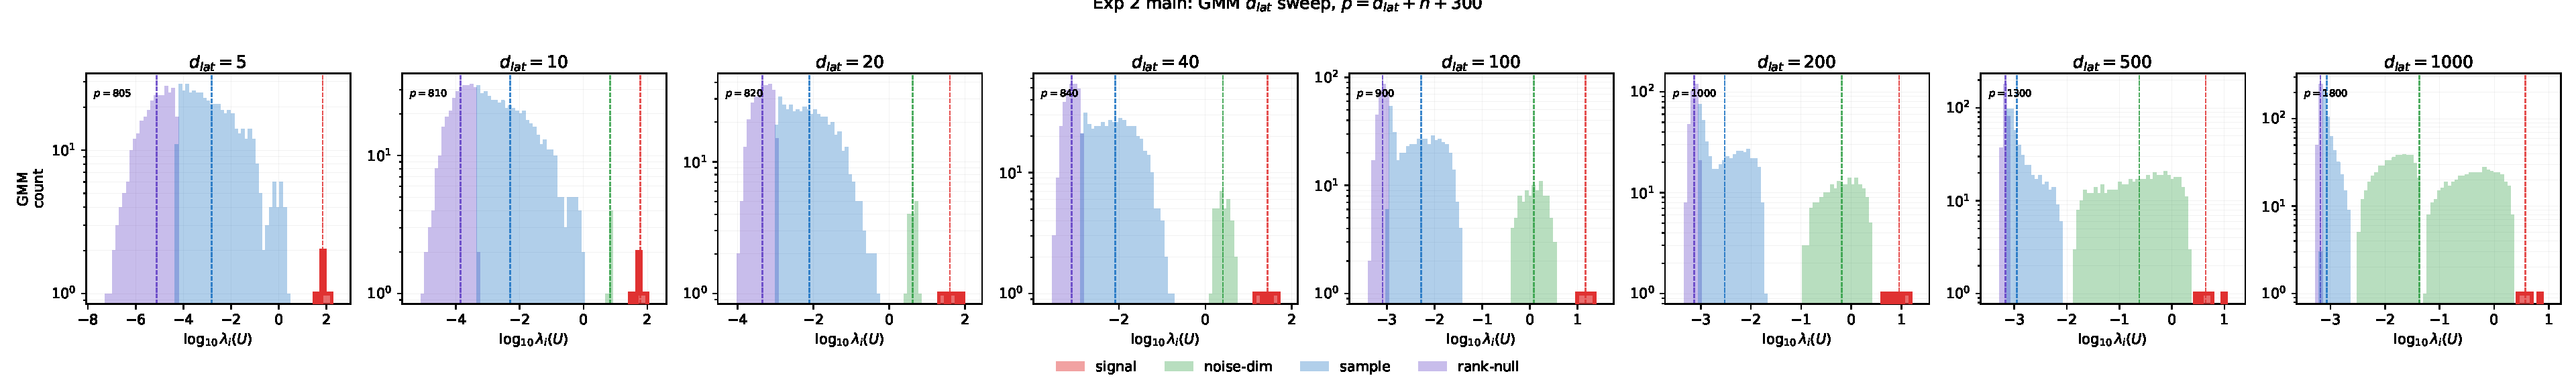
\includegraphics[width=\linewidth]{figures/synthetic_rfnn_exp2_four_bulk.pdf}
  \caption{\textbf{RFNN four-bulk spectrum for the $\dlat$ sweep.}
    A synthetic GMM with fixed $\dint=5$ is embedded into increasing
    $\dlat$. The red signal modes stay fixed in count, while the
    green noise-dimension bulk grows with $\dlat-\dint$ before the
    model reaches the blue sample-specific modes.}
  \label{fig:fourbulk-clean}
\end{figure}

\citet{bonnaire2025} already note (Figure~4, right panel) that
$\rho_2$ develops internal structure when $\Sigmadata$ has multiple
eigenvalues, but at signal-to-null ratio $3{\times}$ they treat it
as a single deformed bulk. The latent-diffusion regime sits at the
opposite extreme ($\sigsig^2/\signoise^2 \approx 10^4$ at
$\signoise = 0.01$, $\approx 4$ at $\signoise = 0.5$): the humps
inside $\rho_2$ separate into well-isolated bulks decades apart,
which is why we count them as distinct.

\begin{figure}[!t]
  \centering
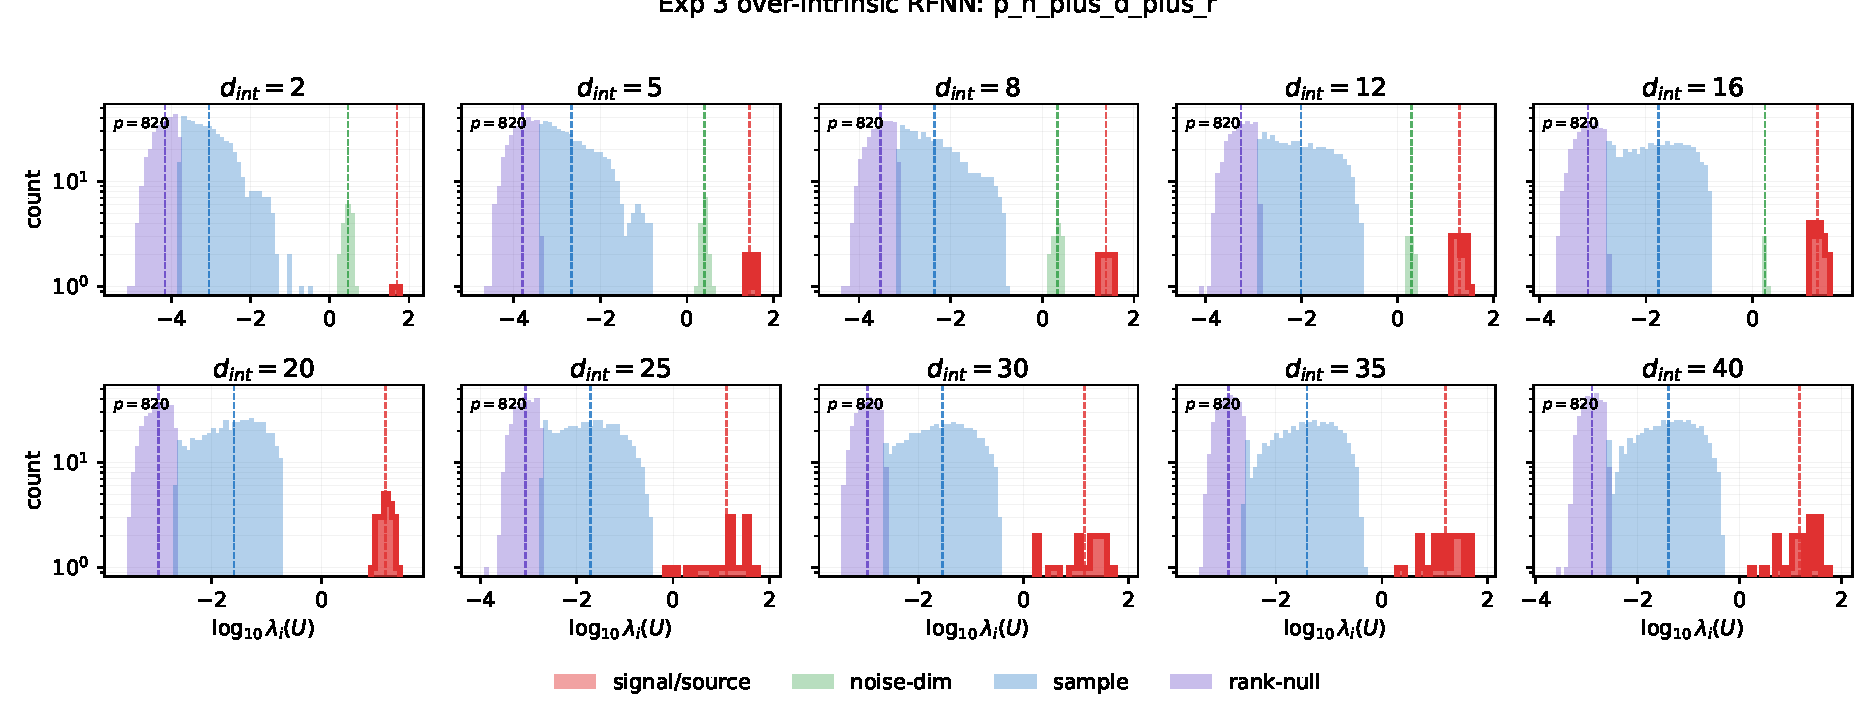
\includegraphics[width=0.95\linewidth]{figures/synthetic_rfnn_exp3_overintrinsic_four_bulk.pdf}
  \caption{\textbf{RFNN Exp-3 source-dimensionality sweep.}
    We fix the observed latent space at $\dlat=20$ and regenerate
    the source GMM for each $\dint$, including over-intrinsic
    cases where the source dimension exceeds the observed latent
    dimension and is randomly compressed. The signal/source block
    grows until $\dint=\dlat$; past that point there is no
    additional observed signal dimension, so the green
    noise-dimension buffer disappears.}
  \label{fig:fourbulk-hist}
\end{figure}

\textbf{Mechanism: a noise-dimension buffer.}
\looseness -1
The RFNN absorbs modes in order of decreasing $\lambda_i$, so the
trajectory traverses the four bulks sequentially: signal bulk
first (defining $\taugen$, $\dlat$-independent at fixed $\sigsig$,
$k$, cluster scale); noise-dim bulk next (additional training time,
no sample-quality benefit); sample bulk last (defining $\taumem$).
Because the buffer grows as $\dlat - \dint$, the larger this
difference, the longer the time before memorization begins, while
$\taugen$ stays fixed. The buffer does not exist in Bonnaire's
isotropic case.

\textbf{What the gen-gap measures.}
\looseness -1
The training set carries two kinds of structure. The data bulks
correspond to \emph{population} structure: directions of variance
that exist in the population and happen to also be visible in the
training sample. The sample bulk corresponds to \emph{null
structure}: directions that look like signal in the $\nsamp$
training points but do not exist in the population. The RFNN
absorbs eigenmodes in order of decreasing $\lambda_i$, so it fits
the population structure first and the null structure later. While
it is fitting population structure, train and test loss drop
together. Once it begins fitting null structure, train loss keeps
dropping but test loss does not, and the gap opens. The gen-gap is
therefore a direct measure of how much null structure the readout
has absorbed, which is why it opens at $\taumem$ and why the
noise-dim buffer also delays its onset: widening the buffer pushes
back the moment when null structure begins to be learned.

\textbf{Decomposing the four-bulk structure.}
The signal and noise-dim bulks of $\Umat$ inherit the block
structure of $\Sigmadata$ directly: $X^\top X / \nsamp$ on the same
training data has $\dint$ large eigenvalues in the signal subspace
and $\dlat - \dint$ small eigenvalues in the null directions,
separated by roughly $\sigsig^2 / \signoise^2$, and the lift by $W$
carries them into the data bulks of $\Umat$ up to a constant from
$W$'s spectrum. The sample and rank-null bulks are feature-space
artifacts of $\nsamp$ training points lifted into
$\pwidth > \dlat$ random features. The buffer mechanism is thus
gradient flow following the data's own variance hierarchy.

% \subsection{Theoretical bounds}
% \label{sec:rfnn-bounds}
%
% \todo{TBD. Candidate directions:}
% \begin{itemize}\itemsep1pt
%   \item \emph{Existence of the noise-dim bulk.} Show that whenever
%     $\dlat > \dint$ and $\sigsig^2 / \signoise^2 \gg 1$, the
%     spectrum of $\Umat$ contains an isolated bulk of size
%     $\dlat - \dint$ inherited from the null block of $\Sigmadata$.
%   \item \emph{Why the noise-dim bulk appears.} Trace the bulk to
%     the rank decomposition of $M_t$ in
%     Appendix~\ref{app:proof-sketch}: the null block of $\Sigmadata$
%     contributes $\dlat - \dint$ eigenvalues at scale
%     $e^{-2t}\signoise^2 + \Delta_t$, which the lift by $W$ carries
%     to a separate bulk of $\Umat$.
%   \item \emph{Bulk-size scaling with $\dlat / \dint$.} Quantify how
%     each of the four bulks grows with $\dlat / \dint$: signal bulk
%     fixed at $\dint$ modes, noise-dim bulk linear in
%     $\dlat - \dint$, sample bulk $\Theta(\nsamp)$, rank-null bulk
%     $\Theta(\pwidth - \dlat - \nsamp)$. Empirical sizes in
%     Table~\ref{tab:bulk-sizes}.
% \end{itemize}

